ProtoDUNE-SP is intended to be a full slice of the DUNE far detector as near as possible to the final DUNE Single Phase design. It will instrument 6 full-size DUNE APAs with 20 FEMB each for a total readout channel count of 15,360 digitized sense wires. Critically, the CE on each APA will be read out via a full CE read out system, via a CE flange and WIEC with 5 WIBs and 1 PTC. Each APA will also have a full Photon Detector readout system installed.

Once each APA has been validated in the Cold Box at CERN, it will be installed in the ProtoDUNE-SP cryostat. Any issues that are discovered either during the Cold Box tests or the ProtoDUNE-SP commissioning and data-taking will be incorporated into the next iteration of the system design for DUNE.

Preliminary results from the ProtoDUNE-SP cold box indicate that the noise performance of the TPC readout will satisfy the DUNE FD noise requirements of ENC < 700e$^-$ on DUNE length wires. The ENC and temperature of APA2 in the Cold Box are shown in Figure~\ref{fig:cb_results}.

\begin{dunefigure}
[ENC (in electrons) and temperature (in degrees Kelvin) as a function of cold cycle time in GN2 for ProtoDUNE-SP APA2. At the lowest temperature of 160K, the wrapped wires measured 480e$^-$ noise and the straight wires 400e$^-$.]
{fig:cb_results}
{ENC (in electrons) and temperature (in degrees Kelvin) as a function of cold cycle time in GN2 for ProtoDUNE-SP APA2. At the lowest temperature of 160K, the wrapped wires measured 480e$^-$ noise and the straight wires 400e$^-$.}
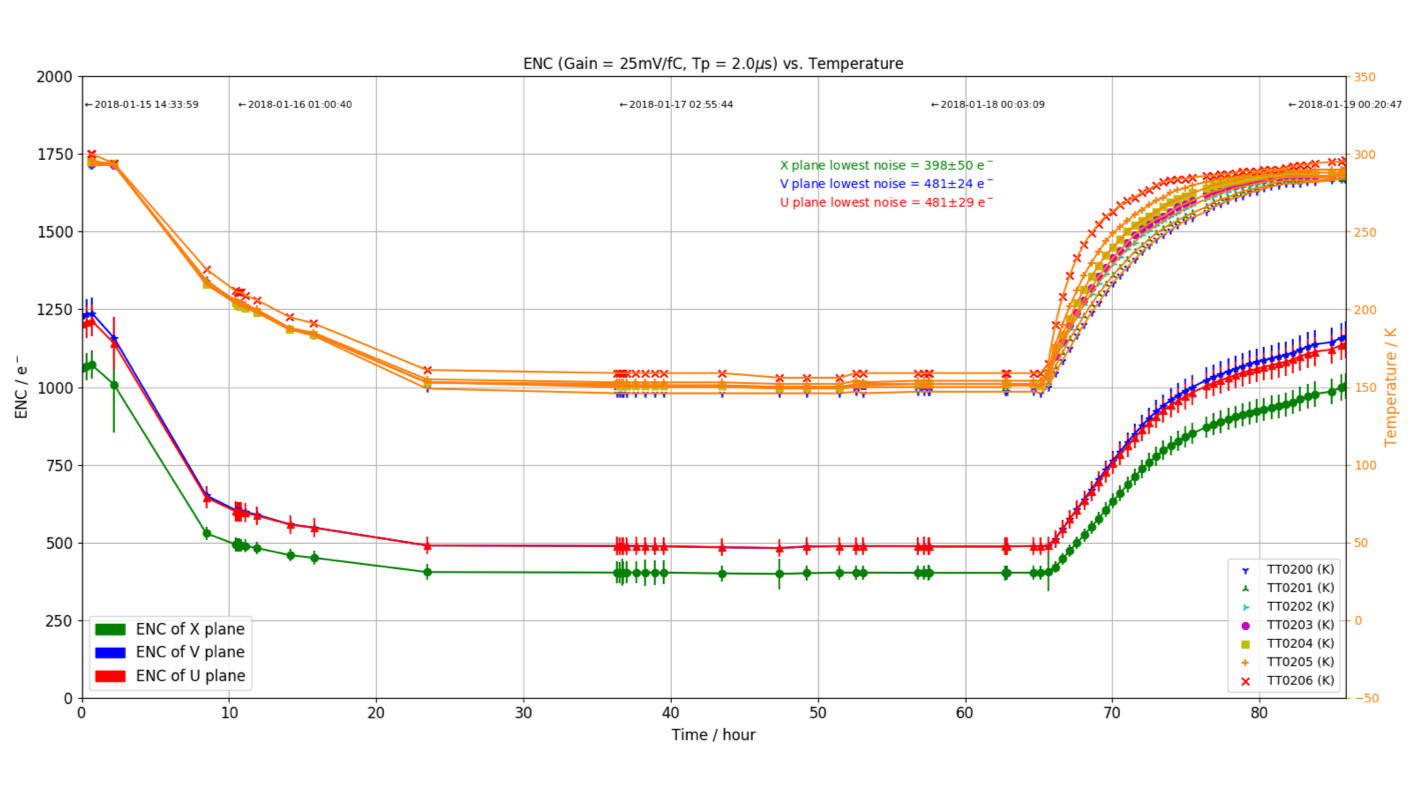
\includegraphics[width=0.9\linewidth]{tpcelec-apa2-results.png}
\end{dunefigure}

Tests have also been done on the ProtoDUNE-SP APA to check for any additional noise introduced on the TPC wire readout by operating the PD system or enabling the wire-bias HV system. So far, no significant increase in the noise on the APA wire readout has been observed when operating these other systems.
